%% LyX 2.2.0 created this file.  For more info, see http://www.lyx.org/.
%% Do not edit unless you really know what you are doing.
\documentclass[spanish,aspectratio=43,oneside,mathserif,notheorems,table]{beamer}
\usepackage[T1]{fontenc}
\usepackage[latin9]{inputenc}
\setcounter{secnumdepth}{3}
\setcounter{tocdepth}{3}
\usepackage{graphicx}

\makeatletter
%%%%%%%%%%%%%%%%%%%%%%%%%%%%%% Textclass specific LaTeX commands.
 % this default might be overridden by plain title style
 \newcommand\makebeamertitle{\frame{\maketitle}}%
 % (ERT) argument for the TOC
 \AtBeginDocument{%
   \let\origtableofcontents=\tableofcontents
   \def\tableofcontents{\@ifnextchar[{\origtableofcontents}{\gobbletableofcontents}}
   \def\gobbletableofcontents#1{\origtableofcontents}
 }

%%%%%%%%%%%%%%%%%%%%%%%%%%%%%% User specified LaTeX commands.
\usetheme[pageofpages=de,% String used between the current page and thetotal page count.
          bullet=circle,% Use circles instead of squares for bullets.
          titleline=true,% Show a line below the frame title.
          alternativetitlepage=true,% Use the fancy title page.
          titlepagelogo=../graphics/logo.png,% Logo for the first page.
          ]{Torino}
% Nouvelle is a green and red alternative to the chameleon color theme.
\usecolortheme{freewilly}
%\usecolortheme{nouvelle}

\newcommand{\monthname}{\ifcase\month\or Enero\or Febrero\or
      Marzo\or Abril\or Mayo\or Junio\or Julio\or Agosto\or Septiembre\or
      Octubre\or Noviembre\or Diciembre\fi}

%Usando para definicion
\usepackage{amsthm}
\setbeamertemplate{theorems}[numbered]
\theoremstyle{definition} 
\newtheorem{definition}{Definici�n}[section]
\usepackage{algpseudocode}

\newcommand{\alertline}{%
 \usebeamercolor[fg]{normal text}%
 \only{\usebeamercolor[fg]{alerted text}}}

\makeatother

\usepackage{babel}
\addto\shorthandsspanish{\spanishdeactivate{~<>}}

\begin{document}

\title{Reconocimiento de Actividades Humanas con un enfoque colaborativo}

\subtitle{Proyecto Final de Grado}

\author{Alberto Gim�nez\\
Santiago Yegros}

\institute{Tutores: Ing. Joaqu�n Lima\\
Ing. Juan Talavera}

\date{Facultad Polit�cnica - \monthname, \the\year}
\makebeamertitle
\begin{frame}

\frametitle<presentation>{Contenido}

\tableofcontents[hideothersubsections]{} 
\end{frame}
%
\AtBeginSection[]
{
	\begin{frame}
		\frametitle{Contenido}        		\tableofcontents[currentsection]
	\end{frame} 
}


\section{Introducci�n}
\begin{frame}{Reconocimiento de Actividades Humanas}

\framesubtitle{Definici�n del Problema}
\begin{overprint}
\onslide<1> 
\begin{quote}
Determinar las acciones o comportamientos de uno o m�s individuos
a partir de datos ambiguos capturados por sensores situados en el
entorno. 
\begin{flushright}
{\small{}\emph{{\small{}{[}Bao and Intille, 2004, Chen et al., 2012, Reyes Ortiz,
2015{]}}}}
\par\end{flushright}{\small \par}
\end{quote}
\onslide<2> 
\begin{block}<2>{Nota}
\emph{}El problema es conocido por sus siglas \structure{HAR} en
ingl�s \emph{(Human Activity Recognition})
\end{block}
\end{overprint}
\begin{center}
\begin{minipage}[t]{0.7\columnwidth}%
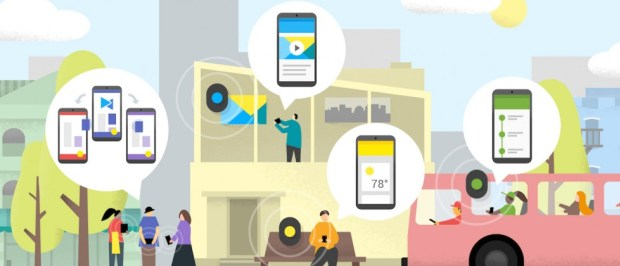
\includegraphics[width=1\textwidth]{intro/graphics/sensor-environment}

\begin{spacing}{0}
\noindent \textcolor{darkgray}{\emph{\tiny{}\copyright Beacons, Google
Developers}}{\tiny \par}
\end{spacing}
%
\end{minipage}
\par\end{center}

\end{frame}
%
\begin{frame}{�Que es HAR?}

\setbeamercovered{transparent}

\framesubtitle{Definici�n del Problema}
\begin{itemize}[<+->]
\item Es un t�pico de investigaci�n multidisciplinario que busca dise�ar
algoritmos para:
\begin{itemize}
\item Capturar movimientos de individuos en interacci�n con su entorno 
\item Realizar aprendizaje e inferencia
\item Proveer informaci�n de contexto 
\end{itemize}
\end{itemize}
\begin{overprint}
\onslide<2> 
\begin{center}
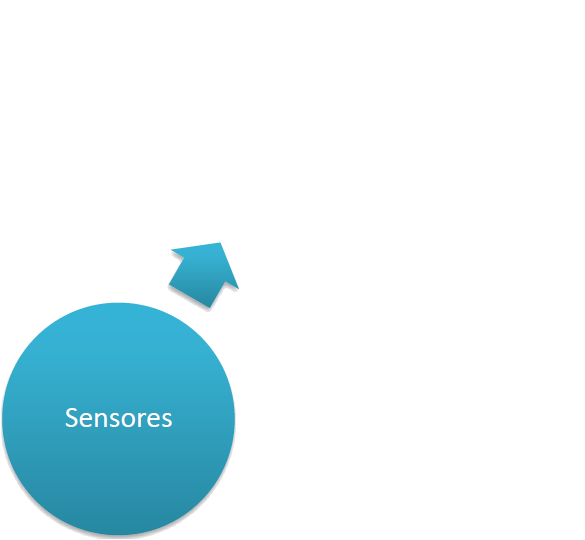
\includegraphics[width=4.5cm]{intro/graphics/areas-1}
\par\end{center}
\onslide<3> 
\begin{center}
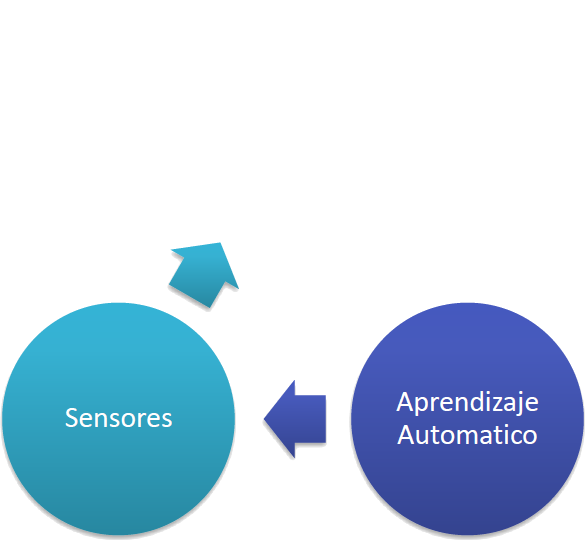
\includegraphics[width=4.5cm]{intro/graphics/areas-2}
\par\end{center}
\onslide<4> 
\begin{center}
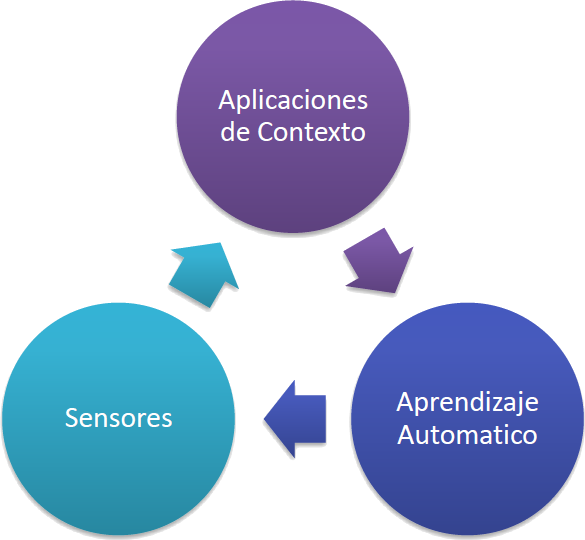
\includegraphics[width=4.5cm]{intro/graphics/areas-3}
\par\end{center}

\end{overprint}
\end{frame}
%
\begin{frame}{Motivaci�n}

\framesubtitle{Definici�n del Problema}

\setbeamercovered{transparent}\setlength\columnsep{0pt}
\begin{columns}

\column{0.5\textwidth}
\begin{itemize}
\item El \structure{contexto} es primordial para los sistemas inteligentes 
\end{itemize}
\begin{spacing}{0.5}

\pause{}
\end{spacing}
\begin{itemize}
\item Avances en tecnolog�as de \structure{computaci�n m�vil} y \structure{sensores} 
\end{itemize}
\begin{spacing}{0.5}

\pause{}
\end{spacing}
\begin{itemize}
\item Uso intensivo de \structure{tel�fonos m�viles modernos} en la vida
diaria.
\end{itemize}
\begin{spacing}{0.5}

\pause{}
\end{spacing}
\begin{itemize}
\item Popularidad de \structure{aplicaciones m�viles} de contexto en 
\begin{itemize}
\item el cuidado personal, 
\item la movilidad y 
\item la asistencia en la vida diaria 
\end{itemize}
\end{itemize}

\column{0.5\textwidth}
\begin{overprint}
\onslide<1> 


\includegraphics[width=1\textwidth]{intro/graphics/context1}

\begin{spacing}{0}
\noindent \emph{\tiny{}\copyright Connected Social Media, Intel}{\tiny \par}
\end{spacing}
\onslide<2> 


\includegraphics[width=1\textwidth]{intro/graphics/sensors}
\onslide<3> 

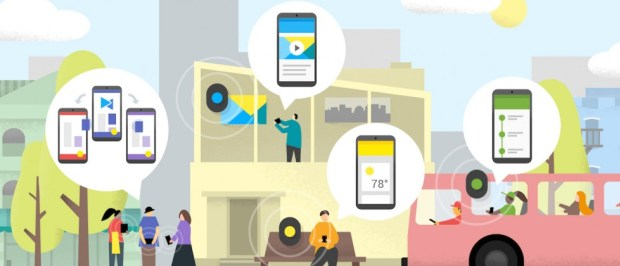
\includegraphics[bb=100bp 0bp 520bp 266bp,clip,width=1\textwidth]{intro/graphics/sensor-environment}

\begin{spacing}{0}
\noindent \emph{\tiny{}\copyright Beacons, Google Developers}{\tiny \par}
\end{spacing}
\onslide<4-> 


\includegraphics[width=1\textwidth]{intro/graphics/mobile-phone}

\begin{spacing}{0}
\noindent \emph{\tiny{}\cc Mobile Dev, Pinterest}{\tiny \par}
\end{spacing}
\end{overprint}
\end{columns}

\end{frame}
%
\begin{frame}{Contexto}

\framesubtitle{Definici�n del Problema}

Medio de interacci�n que representa el estado de la informaci�n f�sica,
emocional, social, entre otros. \emph{{[}Dey and Abowd, 2000{]}}
\begin{uncoverenv}<2>
\begin{columns}[t]

\column{0.5\textwidth}
\begin{itemize}
\item Ubicaci�n 
\item Identidad 
\item Actividad f�sica
\item Tiempo
\item Social
\end{itemize}

\column{0.5\textwidth}
\begin{center}
\textcolor{darkgray}{\emph{\tiny{}}}%
\noindent\begin{minipage}[t]{1\columnwidth}%
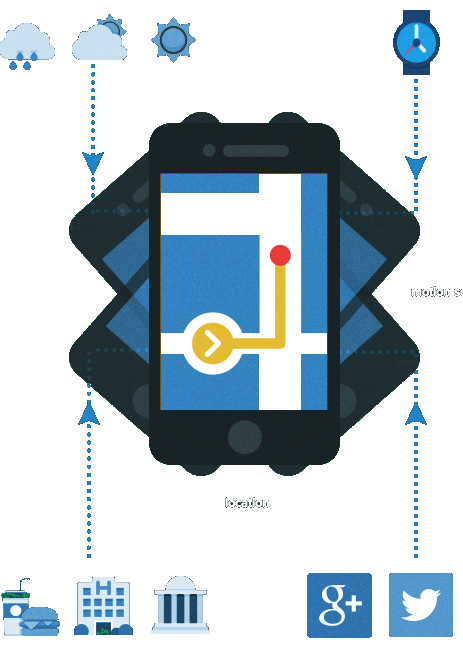
\includegraphics[width=0.65\textwidth]{intro/graphics/context2}\textcolor{darkgray}{\emph{\tiny{}\copyright
Toptal.io}}%
\end{minipage}
\par\end{center}{\tiny \par}

\end{columns}

\end{uncoverenv}

\end{frame}
%
\begin{frame}{HAR en Android}

\framesubtitle{Definici�n del Problema}

En la actualidad \emph{\textbf{\emph{Google Play Services}}} es la
�nica librer�a \structure{HAR} de uso libre para aplicaciones m�viles
de terceros.
\begin{overprint}
\onslide<1> 

\begin{figure}
\caption{Arquitectura de \protect\structure{HAR} en \protect\emph{Android}}

\centering{}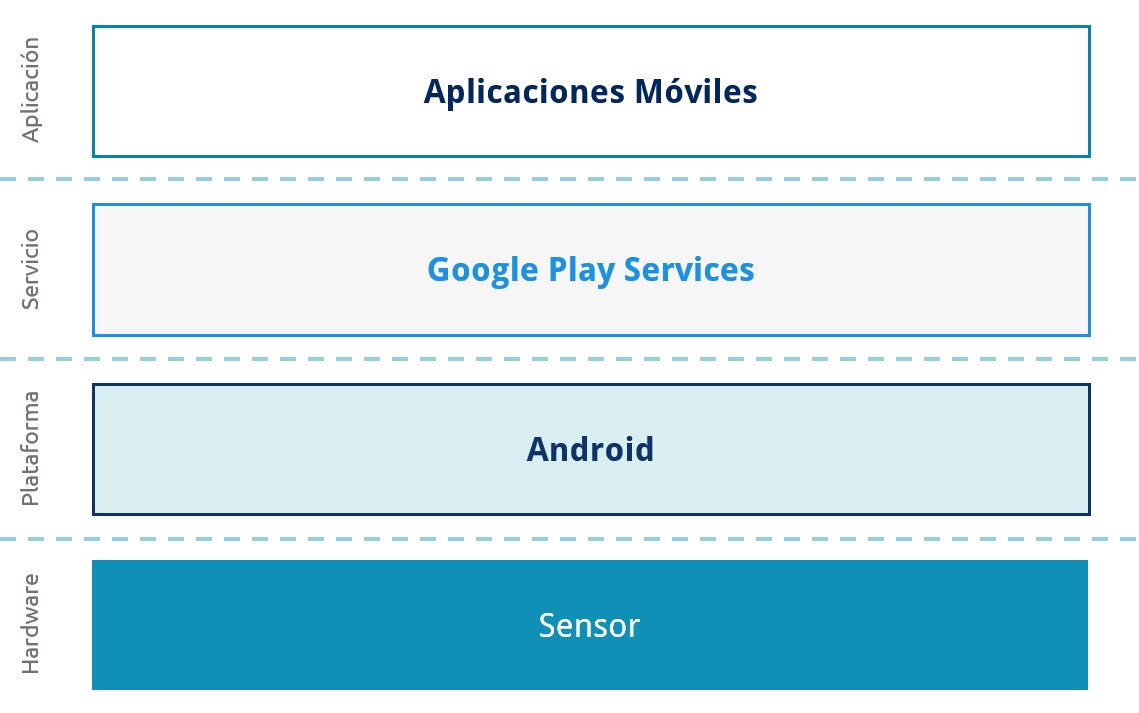
\includegraphics[width=0.65\textwidth]{intro/graphics/har_stack}
\end{figure}

\onslide<2> 
\begin{itemize}
\item No es de c�digo abierto (\structure{open source}).
\item Es de libre utilizaci�n pero no puede ser mejorado y extendido de
forma \structure{colaborativa}.
\item No existe una herramienta de software libre para fines pr�cticos e
investigaci�n equivalente con respecto a \structure{HAR}.
\end{itemize}
\end{overprint}
\end{frame}



\begin{frame}{Propuesta}

\framesubtitle{Alcance}
\begin{center}
Reconocer actividades humanas utilizando tel�fonos m�viles modernos
a partir de una herramienta de c�digo abierto extensible y personalizable
con un enfoque colaborativo
\par\end{center}

\end{frame}
%
\begin{frame}{Actividades Humanas}

\framesubtitle{Alcance}

\setbeamercovered{transparent}
\begin{columns}

\column{0.25\textwidth}
\begin{itemize}
\item Acciones cortas
\end{itemize}
\begin{spacing}{0.5}

\pause{}
\end{spacing}
\begin{itemize}
\item Actividades Simples
\end{itemize}
\begin{spacing}{0.5}

\pause{}
\end{spacing}
\begin{itemize}
\item Actividades Complejas
\end{itemize}
\begin{spacing}{0.5}

\pause{}
\end{spacing}
\begin{itemize}
\item Actividades Colectivas
\end{itemize}

\column{0.75\textwidth}
\begin{center}
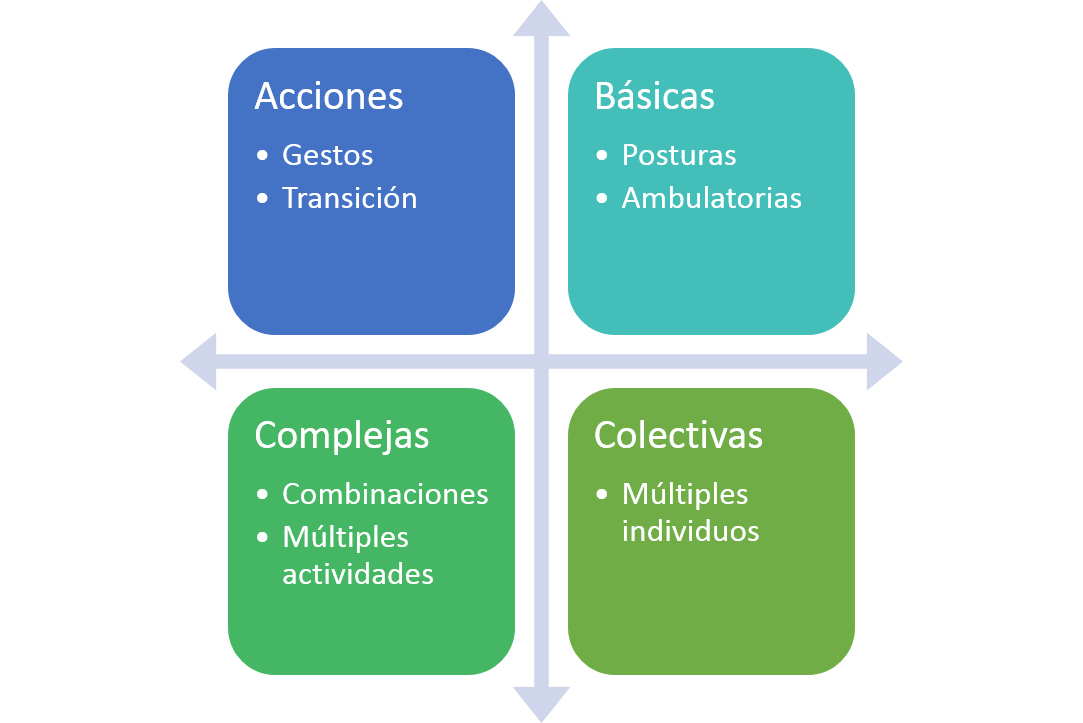
\includegraphics[width=0.95\columnwidth]{propuesta/graphics/actividades}
\par\end{center}

\begin{flushright}
{\small{}\emph{{\small{}{[}Chen et al., 2012, Reyes Ortiz, 2015{]}}}}
\par\end{flushright}{\small \par}

\end{columns}

\end{frame}
%
\begin{frame}{Actividades Humanas}

\framesubtitle{Alcance}

\resizebox{0.75\textwidth}{!}{

\noindent\begin{minipage}[t]{1\columnwidth}%
\begin{tabular}{l|>{\raggedright}p{5cm}|>{\raggedright}m{6cm}}
\textbf{Grupo}  & \textbf{Actividades}  & \textbf{�reas de Aplicaci�n}\tabularnewline
\hline 
Posturas & Sentado

Parado

Acostado & Medicina, Cuidado Personal, Asistencia en vida diaria\tabularnewline
\hline 
Ambulatorias  & Caminar

Correr

Quieto

Subir y descender escaleras & Cuidado Personal, Entretenimiento\tabularnewline
\hline 
Transporte  & \noindent En bus o autom�vil

\noindent En bicicleta & Conmutar, Seguridad\tabularnewline
\hline 
Cotidianas & \noindent Comer

\noindent Beber

\noindent Trabajar en la PC

\noindent Mirar TV

\noindent Leer un libro  & Asistencia en la vida diaria, Ambientes inteligentes\tabularnewline
\end{tabular}%
\end{minipage}

}
\end{frame}




\section{Metodolog�a y Sistemas HAR}

\begin{frame}[t]{Definici�n Te�rica}
\framesubtitle{Metodolog�a HAR}

\begin{block}{Problema HAR} 

Dado un conjunto $W=\{w_{0},...,w_{m-1}\}$ con $m$ ventanas de tiempo \\~\ 

donde cada $w_{j}$ contiene series de tiempo $S_{j}=\{s_{j,0},...,s_{j,k-1}\}$ para $k$ se�ales \\~\ \par

Y un conjunto $A\text{=}\{\mathrm{a}_{0},...,\mathrm{a}_{n-1}\}$ de $n$ actividades \\~\

El objetivo es encontrar $\mathbf{  F\colon S_{j}\rightarrow A }$ para todos los $S_{j}$ en cada $w_{j}$ \\~\
\end{block}

\end{frame}
%
\begin{frame}{Proceso de aprendizaje}
\framesubtitle{Metodolog�a HAR}
	\begin{center}
		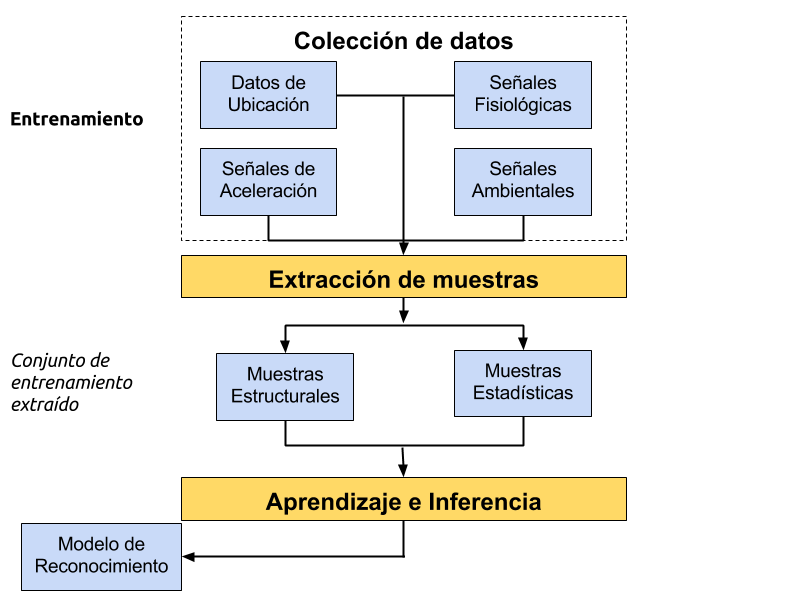
\includegraphics[width=8cm]{propuesta/graphics/har-3}
		\par
	\end{center}
\end{frame}
%
\begin{frame}{Proceso de evaluaci�n}
\framesubtitle{Metodolog�a HAR}
	\begin{center}
		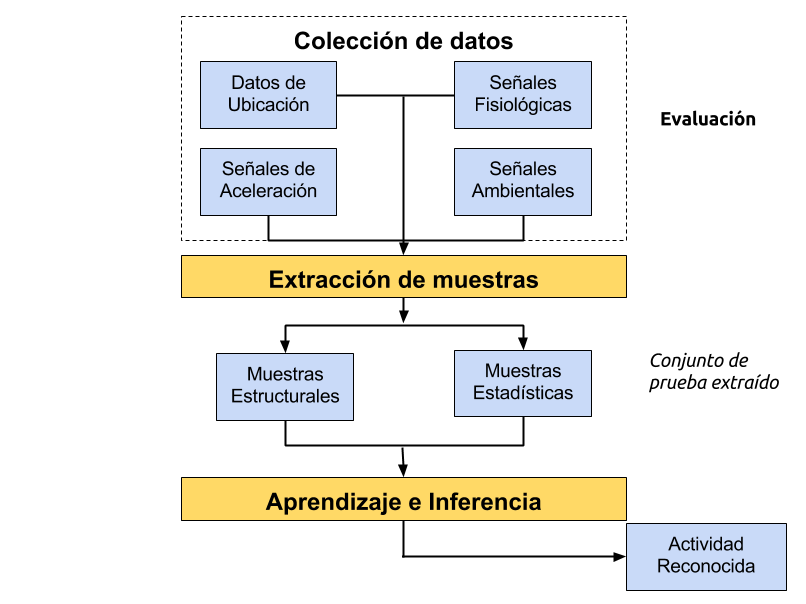
\includegraphics[width=8cm]{propuesta/graphics/har-6}
		\par
	\end{center}
\end{frame}
%
\begin{frame}{Proceso HAR}
\framesubtitle{Metodolog�a HAR}
	\begin{center}
		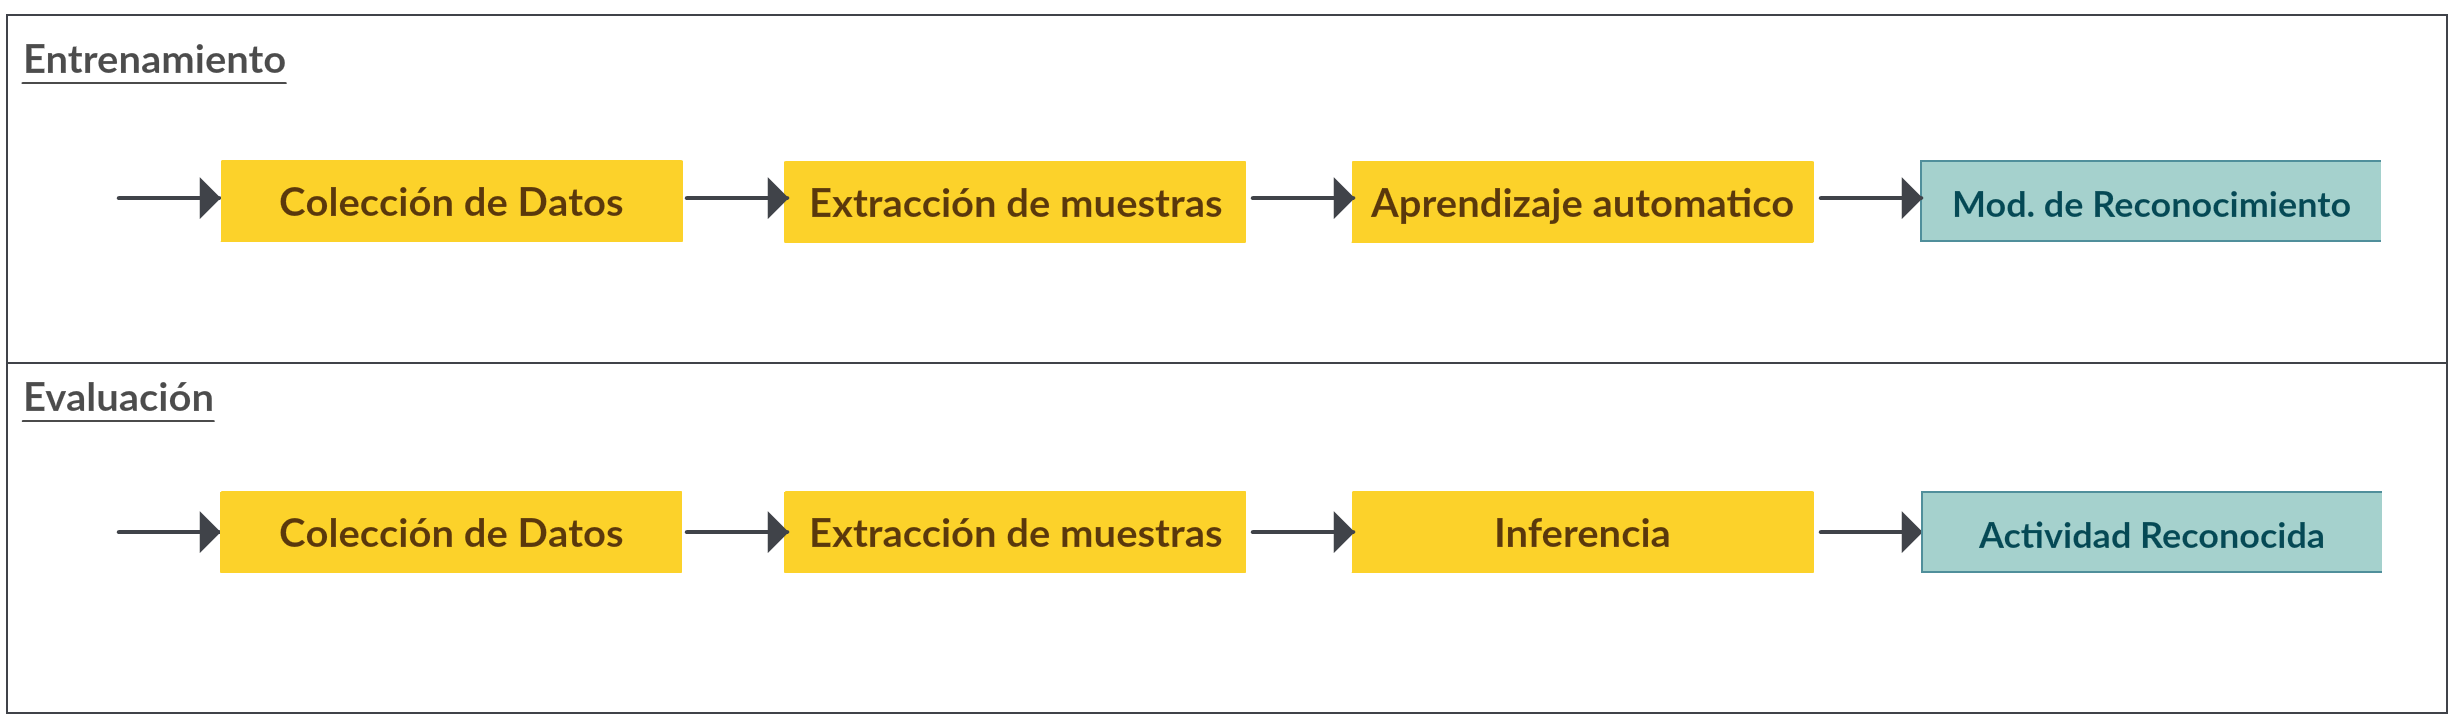
\includegraphics[width=11.5cm]{propuesta/graphics/metodologia_har}
		\par
	\end{center}
\end{frame}
%
\begin{frame}{Colecci�n de Datos}
\framesubtitle{Metodolog�a HAR}
El primer paso es recolectar se�ales obtenidas de sensores unidos al cuerpo (cintura, mu�eca, muslos, etc) realizando alguna actividad de inter�s.

\begin{center}
\resizebox{\linewidth}{!}{
\begin{tabular}{|c|c|c|c|c|c|c|c|}
	\hline 
	\multicolumn{8}{|c|}{Sensores} \\ 
	\hline 
	\multicolumn{2}{|c|}{Movimiento}	& \multicolumn{2}{c|}{Posici�n} 	& \multicolumn{2}{c|}{Ambientales}  	& \multicolumn{2}{c|}{Fisiol�gicas}  		\\ 
	\hline 
	
\includegraphics[width=0.05\textwidth]{propuesta/graphics/acelerometro} 	& Acelerometro 		&
	
\includegraphics[width=0.04\textwidth]{propuesta/graphics/barometro}		& Bar�metro			&
	
\includegraphics[width=0.05\textwidth]{propuesta/graphics/camera}			& Camara			&
	
\includegraphics[width=0.05\textwidth]{propuesta/graphics/ritmo_cardiaco}	& Ritmo Card�aco	
	\\
	
\includegraphics[width=0.05\textwidth]{propuesta/graphics/giroscopio} 		& Giroscopio 		&
	
\includegraphics[width=0.05\textwidth]{propuesta/graphics/gps}				& GPS				&
	
\includegraphics[width=0.05\textwidth]{propuesta/graphics/microfono}		& Micr�fono			&
	
\includegraphics[width=0.05\textwidth]{propuesta/graphics/temperatura}		& Temperatura		
	\\
	
\includegraphics[width=0.05\textwidth]{propuesta/graphics/magnetometro} 	& Magnet�metro		&
	
\includegraphics[width=0.05\textwidth]{propuesta/graphics/wifi}				& WIFI				&
	
\includegraphics[width=0.05\textwidth]{propuesta/graphics/luz}				& Luz				&
																				&  						
	\\
	
\includegraphics[width=0.05\textwidth]{propuesta/graphics/pedometro}		& Pod�metro			&	
	
\includegraphics[width=0.05\textwidth]{propuesta/graphics/gsm}				& GSM				&
	
\includegraphics[width=0.05\textwidth]{propuesta/graphics/proximidad}		& Proximidad		&	
																				&					
	\\
	\hline 
\end{tabular}
} % fin del resize
\end{center}
\end{frame}
%
\begin{frame}{Extracci�n de Muestras}
\framesubtitle{Metodolog�a HAR}
	\begin{itemize}
		\setlength\itemsep{1em}
		\item El siguiente paso es el procesamiento de las se�ales obtenidas por los sensores y extraer las caracter�sticas relevantes de los datos sin procesar.
		\item El procesamiento de muestra se basa en cuatro tareas distintas:
		\begin{itemize}
			\item Etiquetado.
			\item Suavizado.
			\item Muestreo.
			\item Extracci�n de Caracter�sticas.
		\end{itemize}
	\end{itemize}
\end{frame}
%
\begin{frame}{Extracci�n de Muestras}
\framesubtitle{Metodolog�a HAR}
\begin{columns}
	
\column{4cm}
	\begin{itemize}[<+->]
		\setlength\itemsep{1em}
		\item \underline{Etiquetado}: Los datos de los sensores se deben recopilar y etiquetar.
		\item \underline{Suavizado}: Los sensores electr�nicos pueden introducir cierta inestabilidad en la se�al (jitter) para reducir esto se aplica uno o mas filtros. 
	\end{itemize}


\column{6cm}
	\begin{overprint}
		\onslide<1> 
		\begin{center}
			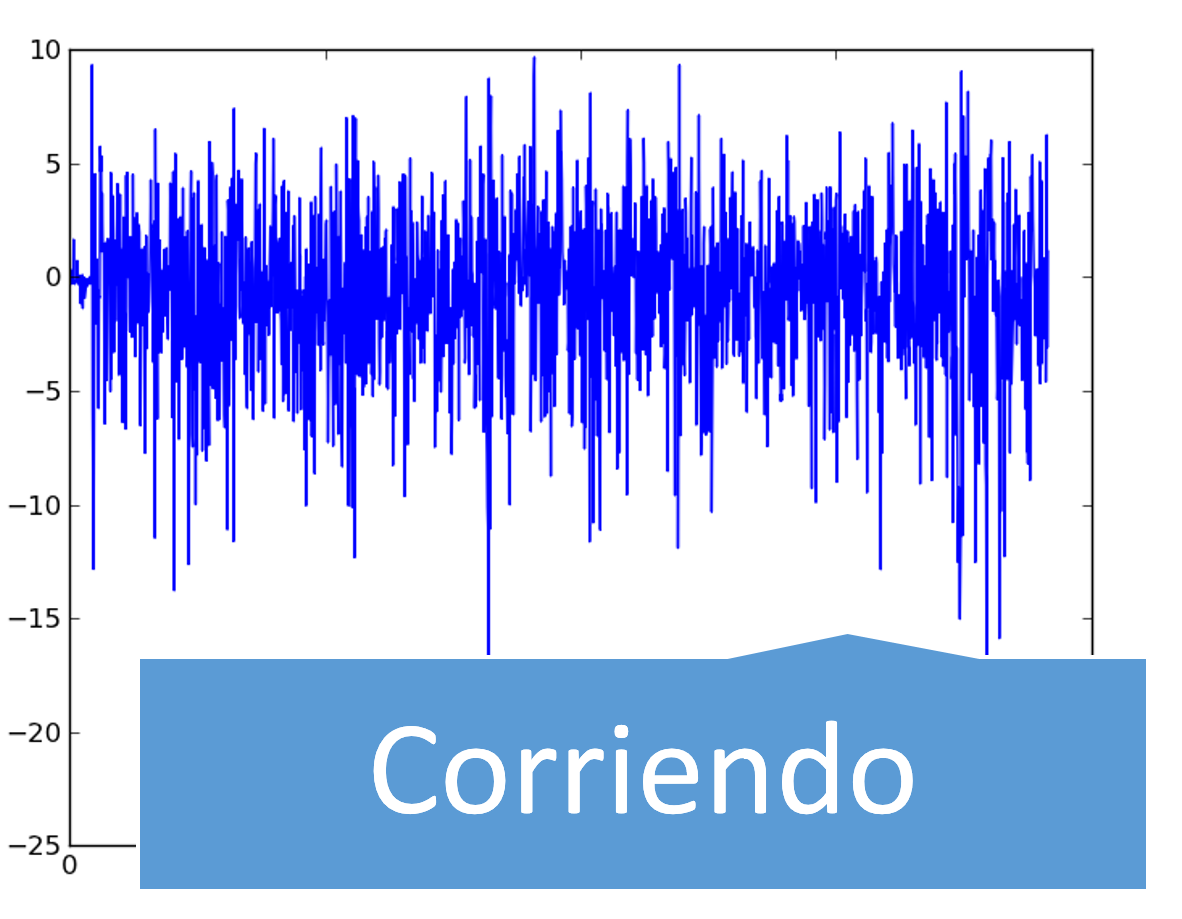
\includegraphics[width=\textwidth]{propuesta/graphics/labelled}
			\par
		\end{center}
		\onslide<2> 
		\begin{center}
			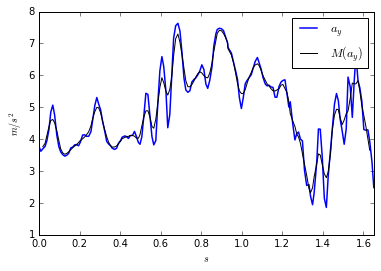
\includegraphics[width=\textwidth]{propuesta/graphics/moving_average}
			\par
		\end{center}
		
	\end{overprint}
\end{columns}
\end{frame}
%
\begin{frame}{Extracci�n de Muestras}
\framesubtitle{Metodolog�a HAR}
\begin{columns}
	
\column{5.2cm}
	\begin{itemize}[<+->]
		\setlength\itemsep{1em}
		\item \underline{Muestreo}: Los datos colectados se segmentan en ventanas de tiempo discretas.
		\item \underline{Extracci�n de Caracter�sticas}: El proceso de extracci�n consiste en extraer valores caracter�sticos en cada ventana de tiempo.
	\end{itemize}

\column{4.8cm}
	\begin{overprint}
	\onslide<1> 
	\begin{center}
		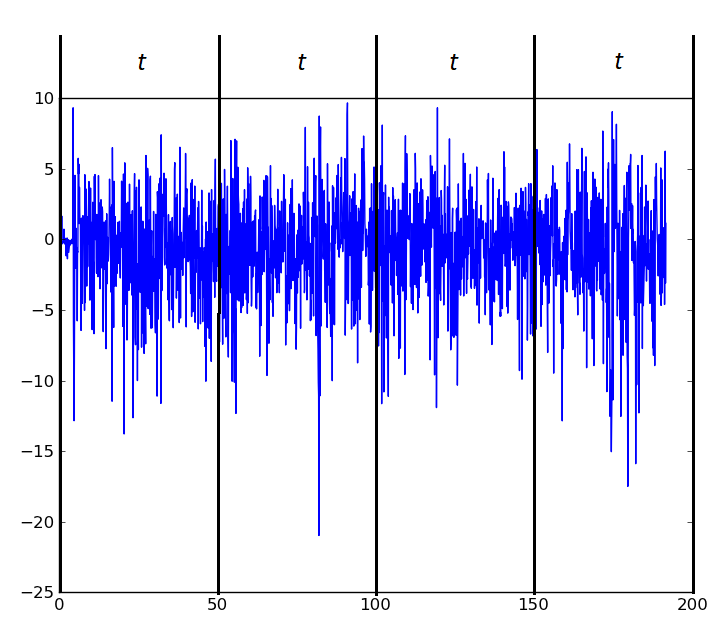
\includegraphics[width=5.2cm]{propuesta/graphics/muestreo}
		\par
	\end{center}
	\onslide<2> 
	\begin{center}
		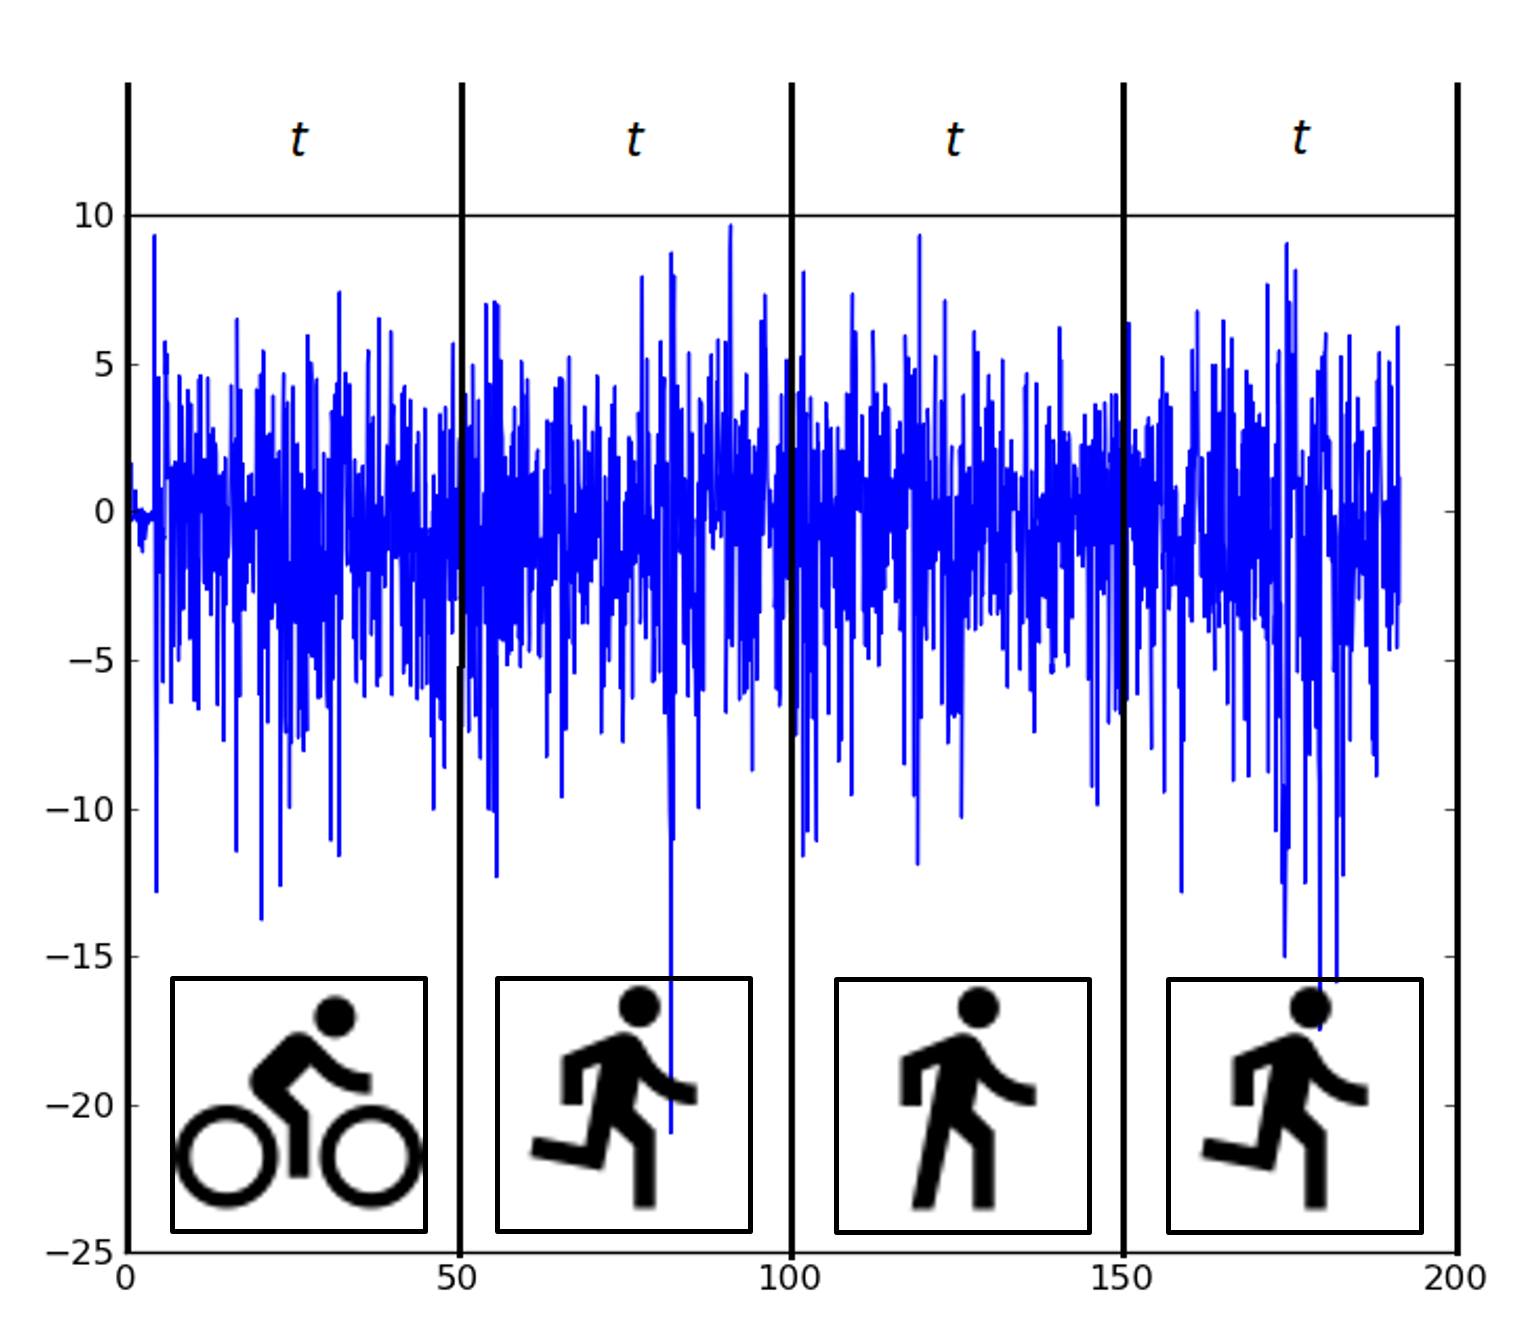
\includegraphics[width=5.2cm]{propuesta/graphics/muestreo_con_act}
		\par
	\end{center}
	\end{overprint}

\end{columns}
\end{frame}
%
\begin{frame}{Inferencia}
\framesubtitle{Metodolog�a HAR}	
La extracci�n se realiza en funci�n a cada muestra $S$ de entrada. Las m�tricas estad�sticas con respecto al tiempo y frecuencia utilizadas son:
\par
\begin{table}
\centering
\resizebox{7cm}{!}{
	\begin{tabular}{|l|l|}
		\hline 
		Funci�n & M�trica \tabularnewline
		\hline 
		\hline 
		\texttt{mean(s)} 			& Media Aritm�tica			\tabularnewline
		\hline 
		\texttt{std(s)} 			& Desviaci�n est�ndar \tabularnewline
		\hline 
		\texttt{max(s)} 			& Valor m�ximo \tabularnewline
		\hline 
		\texttt{min(s)} 			& Valor m�nimo \tabularnewline
		\hline 
		\texttt{skewness(s)} 		& Asimetr�a \tabularnewline
		\hline 
		\texttt{kurtosis(s)} 		& Kurtosis \tabularnewline
		\hline 
		\texttt{energy(s)} 			& Energ�a \tabularnewline
		\hline 
		\texttt{entropy(s)} 		& Entrop�a \tabularnewline
		\hline 
		\texttt{irq(s)} 			& Rango intercuartil \tabularnewline
		\hline 
		\texttt{autoregression(s)} 	& Coeficientes autorregresivos \tabularnewline
		\hline 
		\texttt{meanFreq(s)} 		& Promedio en frecuencia \tabularnewline
		\hline 
	\end{tabular}
	\par
}
\end{table}
\end{frame}
%
\begin{frame}{Aprendizaje e inferencia}
\framesubtitle{Metodolog�a HAR}	
\begin{itemize}
	\setlength\itemsep{1em}
	\item El objetivo principal del algoritmo es clasificar los datos desconocidos en funci�n a muestras obtenidas.
	\item Hay muchos algoritmos de clasificaci�n: 
	\begin{itemize}
		\item \alert<2>{Arboles de Decisi�n}
		\item SVM
		\item Clasificadores de Bayes, 
		\item Modelos de Markov
		\item Redes Neuronales y otros.
	\end{itemize}
\end{itemize}
\end{frame}
%
\begin{frame}{�rbol de Decisi�n}
\framesubtitle{Metodolog�a HAR}	
\begin{columns}
	
\column{0.57\textwidth}
	\begin{itemize}[<+->]
		\item M�todo de aprendizaje predictivo sobre un conjunto de instancias etiquetadas.
		\item Cada nodo interno denota una prueba de un atributo, y cada nodo hoja es una etiqueta o clase.
		\item Para su construcci�n se utiliza criterio de proporci�n de ganancia.
		\item Simple de Implementar y tiene un bajo consumo de energ�a.
	\end{itemize}
	
	
\column{0.43\textwidth}
	\begin{overprint}
		\onslide<1-5> 
		\begin{center}
			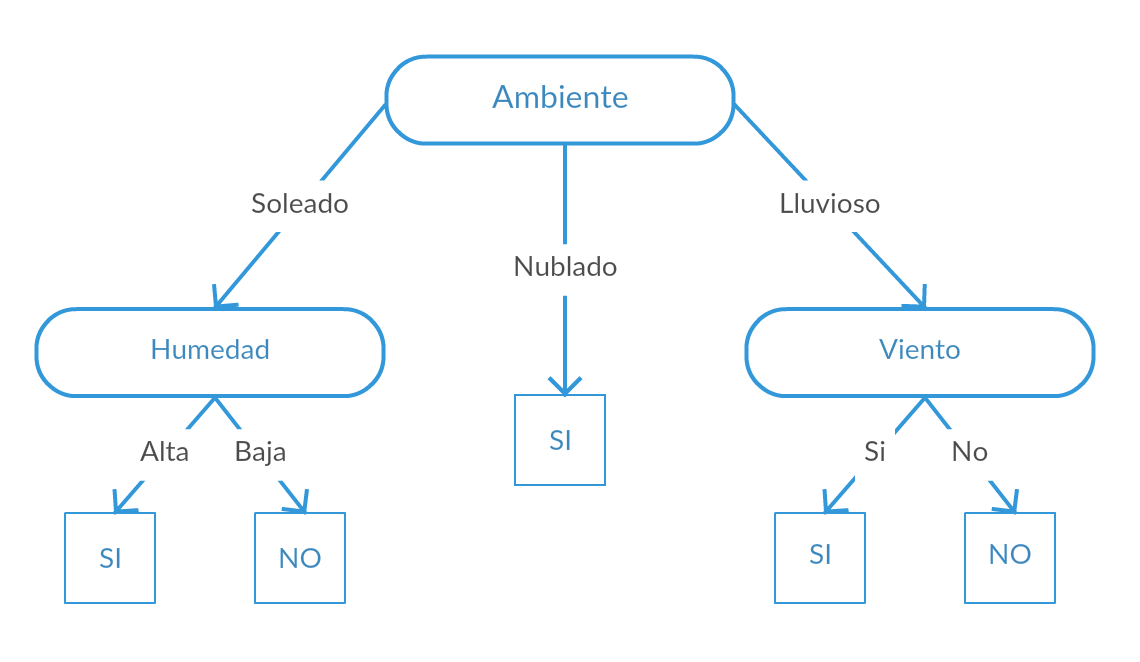
\includegraphics[width=\textwidth]{propuesta/graphics/dtree}
			\par
		\end{center}
		\emph{\footnotesize{}Algoritmos C4.5 (Implementaci�n Java j48 de WEKA)}{\footnotesize \par}

	\end{overprint}
\end{columns}
\end{frame}
%



\section{Sistemas HAR}
\begin{frame}{Sistemas HAR}

\framesubtitle{Aplicaciones de Contexto}

\setbeamercovered{transparent}
\begin{itemize}
\item Aplicaciones cuyo medio de interacci�n incluye al contexto.
\end{itemize}

\pause{}
\begin{itemize}
\item El contexto es el estado acerca de la informaci�n
\begin{itemize}
\item f�sica,
\item emocional,
\item social, entre otros
\end{itemize}
\end{itemize}

\pause{}
\begin{itemize}
\item La computaci�n m�vil y ubicua es sin�nimo de dinamismo en el contexto
\end{itemize}

\pause{}
\begin{itemize}
\item Los tipos de contexto comunes en la computaci�n m�vil son: 
\begin{itemize}
\item la ubicaci�n, 
\item la identidad, 
\item la actividad 
\item y el tiempo
\end{itemize}
\end{itemize}
\end{frame}
%
\begin{frame}<article>{Sistemas HAR}

\framesubtitle{Prop�sito del sistema}

\setbeamercovered{transparent}
\begin{itemize}
\item Proveer un componente para el desarrollo de aplicaciones de contexto. 
\end{itemize}

\pause{}
\begin{itemize}
\item Reconocer actividades realizadas rutinariamente de diferentes maneras, 
\begin{itemize}
\item por diferentes usuarios y 
\item en diferentes contextos.
\end{itemize}

\pause{}
\item Reconocer actividades mediante el uso de sensores.
\end{itemize}

\pause{}
\begin{itemize}
\item Ser portado oportunamente como atuendo para los usuarios (\emph{Wearable})
\end{itemize}
\end{frame}
%
\begin{frame}{Sistemas HAR}

\framesubtitle{Dise�o del sistema}

\setbeamercovered{transparent}
\begin{itemize}
\item Arquitectura basada en aplicaciones de aprendizaje autom�tico.
\end{itemize}

\pause{}
\begin{itemize}
\item Componentes principales
\begin{itemize}
\item un \structure{recolector} de medidas 
\item un \structure{procesador} de muestras 
\item un \structure{clasificador} de actividades
\end{itemize}
\end{itemize}

\pause{}
\begin{itemize}
\item Metodolog�a operativa
\begin{itemize}
\item Aprendizaje fuera de linea (\emph{off-line})
\item Clasificaci�n en linea (\emph{on-line})
\end{itemize}
\end{itemize}
\begin{center}
\visible<2->{\begin{center}
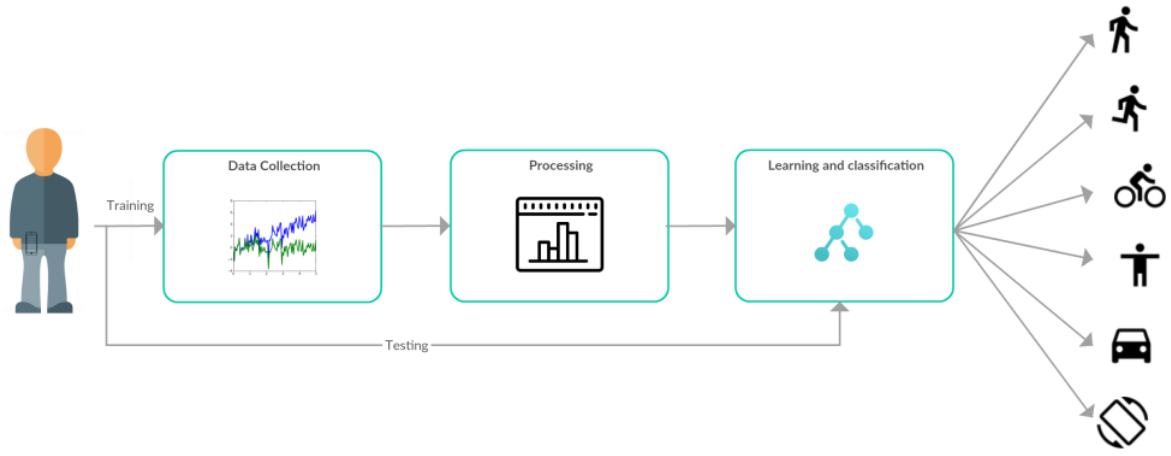
\includegraphics[width=0.6\textwidth]{../capitulo-2/graphics/harsystem2}
\par\end{center}}
\par\end{center}

\end{frame}
%
\begin{frame}{Sistemas HAR}

\framesubtitle{Componentes del sistema}

\setbeamercovered{transparent}
\begin{columns}

\column{0.25\textwidth}
\begin{itemize}
\item Recolector
\begin{itemize}
\item Sensor
\item Registro
\end{itemize}
\end{itemize}

\pause{}
\begin{itemize}
\item Procesador
\begin{itemize}
\item Filtro
\item Extracci�n
\end{itemize}
\end{itemize}

\pause{}
\begin{itemize}
\item Clasificador
\begin{itemize}
\item Aprendizaje
\item Clasificaci�n
\end{itemize}
\end{itemize}

\column{0.75\textwidth}

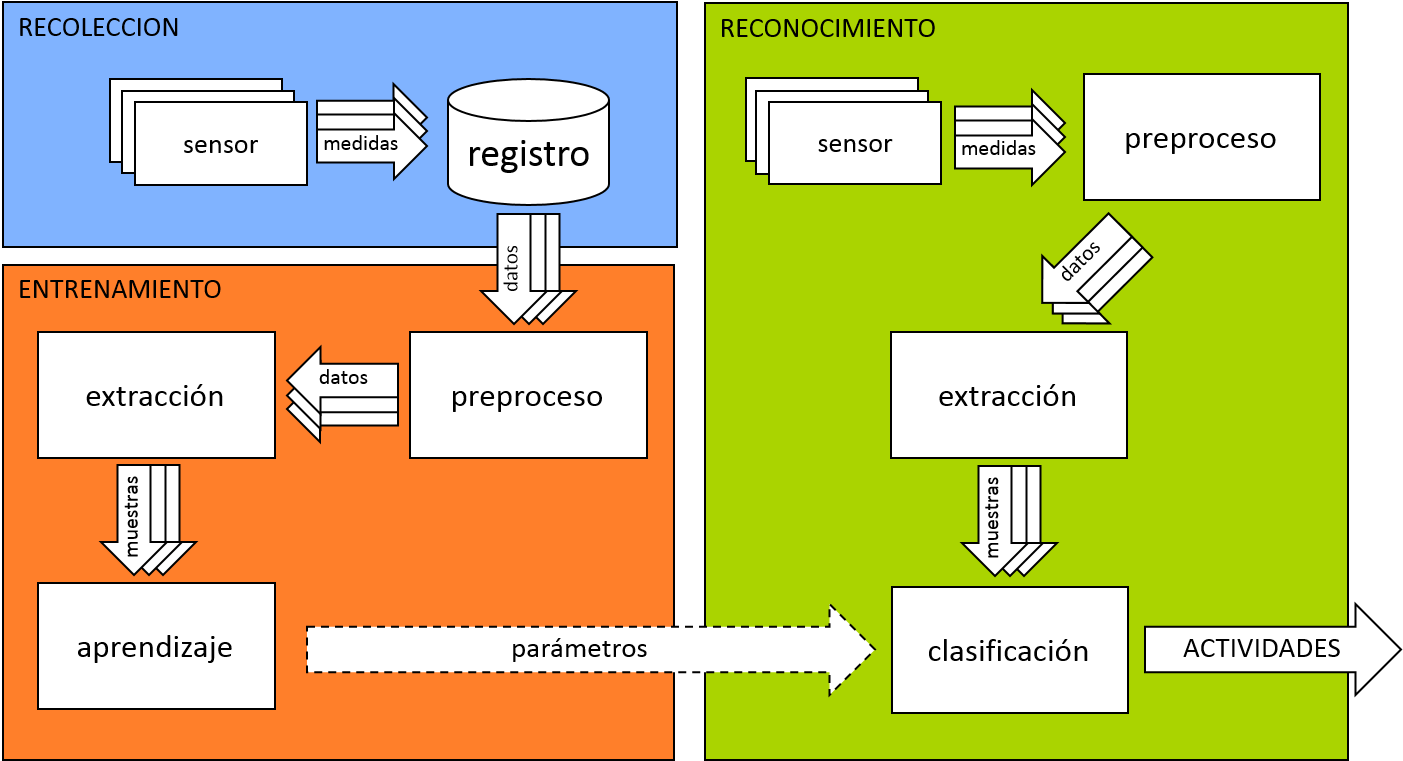
\includegraphics[width=1\columnwidth]{propuesta/graphics/harsystem}
\end{columns}

\end{frame}


\section{HAR en Android}
\begin{frame}{HARDroid}

\framesubtitle{HAR en Android}

\setbeamercovered{transparent}
\begin{columns}

\column{0.4\textwidth}
\begin{itemize}
\item \textbf{HARDroid} 
\begin{itemize}
\item Servicio Reconocedor
\item Clasificador din�mico
\end{itemize}
\begin{spacing}{0.5}

\pause{}
\end{spacing}
\item \textbf{ActivitySurvey}
\begin{itemize}
\item Cliente de Reconocimiento
\item Encuesta guiada
\end{itemize}
\begin{spacing}{0.5}

\pause{}
\end{spacing}
\item \textbf{Backend C4.5} 
\begin{itemize}
\item Servicio web de recolecci�n
\item Aprendizaje en-linea
\end{itemize}
\end{itemize}

\column{0.6\textwidth}
\begin{overprint}
\onslide<1> 
\begin{center}
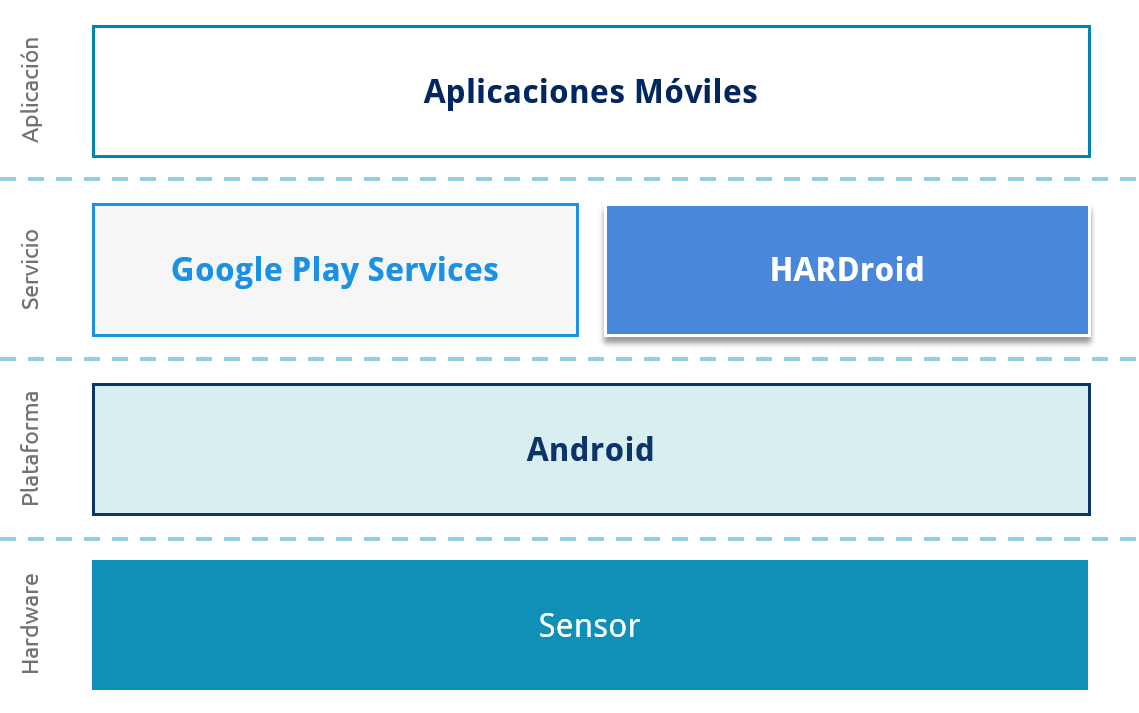
\includegraphics[width=1\columnwidth]{propuesta/graphics/hardroid_stack1}
\par\end{center}
\onslide<2> 
\begin{center}
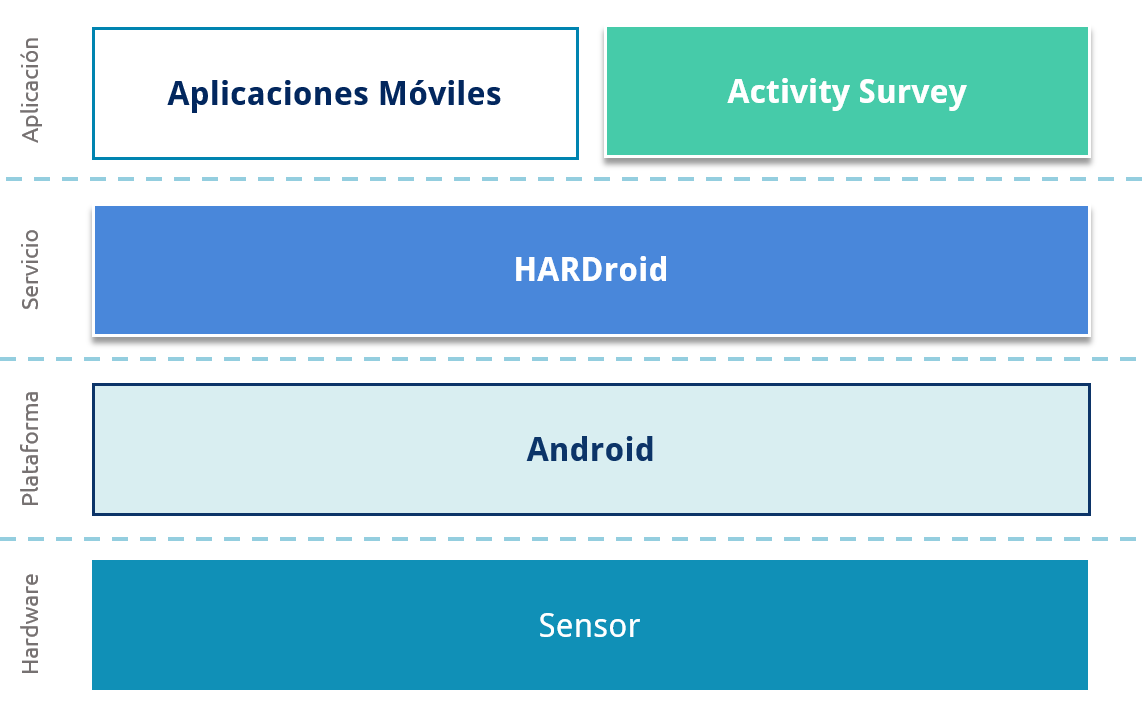
\includegraphics[width=1\columnwidth]{propuesta/graphics/hardroid_stack2}
\par\end{center}
\onslide<3> 
\begin{center}
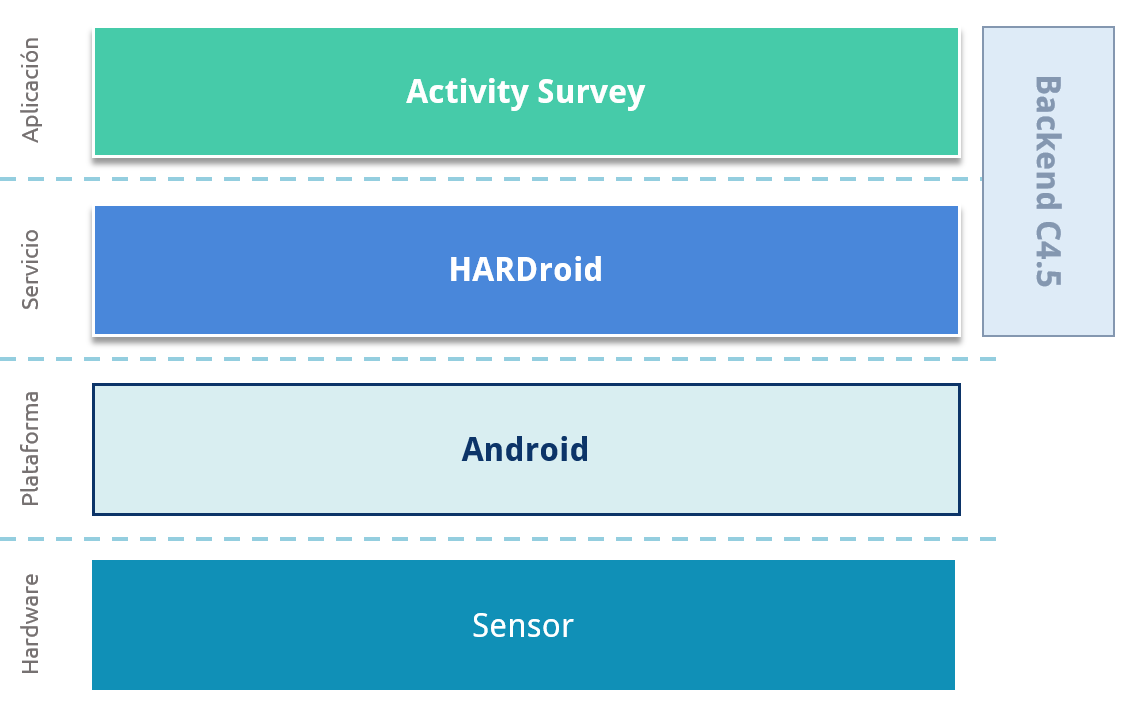
\includegraphics[width=1\columnwidth]{propuesta/graphics/hardroid_stack3}
\par\end{center}

\end{overprint}
\end{columns}

\end{frame}
%
\begin{frame}{HARDroid Colaborativo}

\framesubtitle{HAR en Android}
\begin{center}
\begin{figure}
\begin{centering}
\caption{Proceso colaborativo de mejora continua}
\par\end{centering}
\begin{overprint}
\onslide<1> 
\begin{centering}
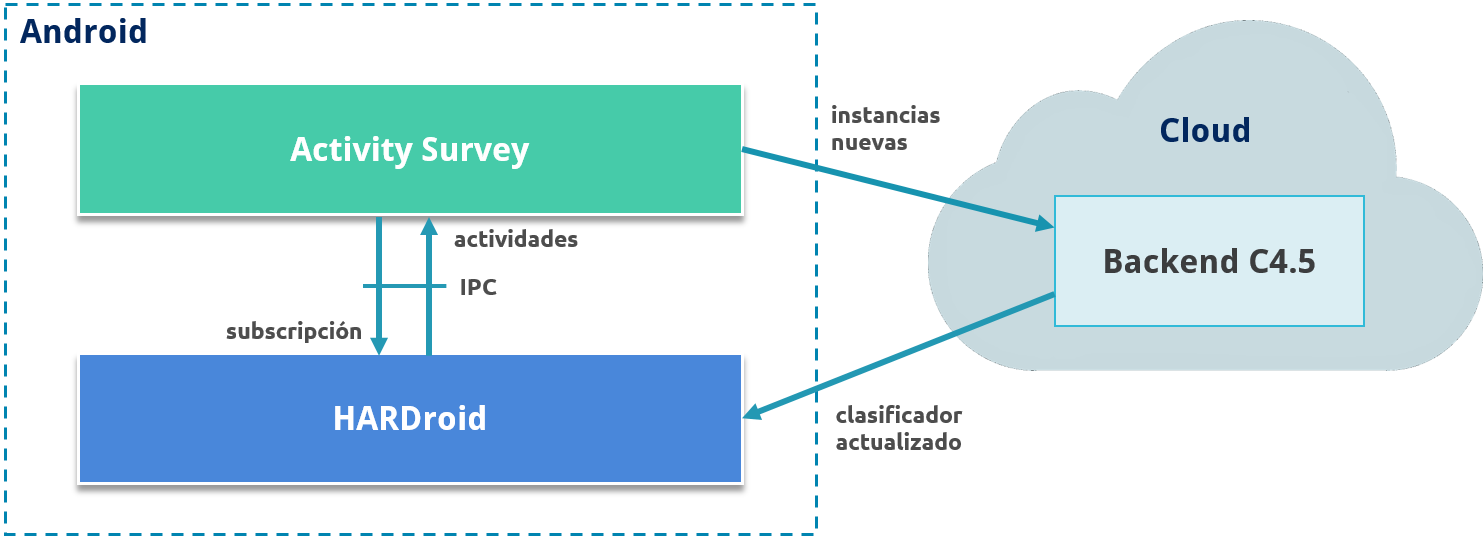
\includegraphics[width=1\columnwidth]{propuesta/graphics/hardroid_colab1}
\par\end{centering}
\onslide<2> 
\begin{centering}
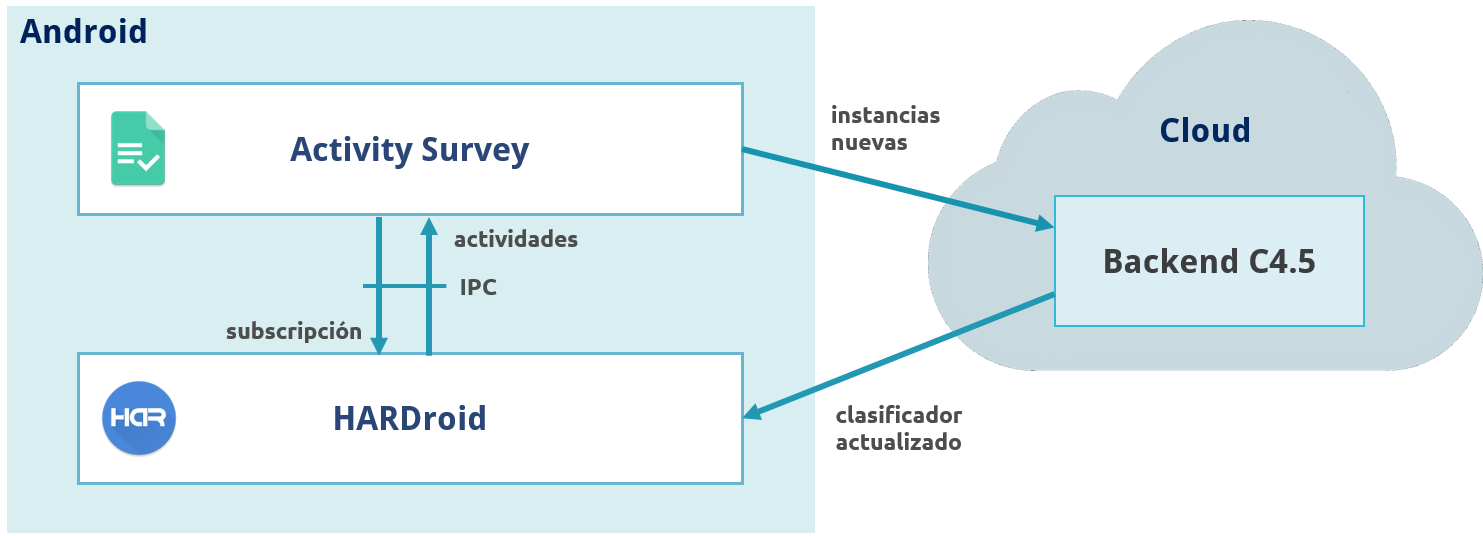
\includegraphics[width=1\columnwidth]{propuesta/graphics/hardroid_colab2}
\par\end{centering}
\centering{}\emph{Disponible en} \structure{\begin{center}
Google Play Store
\par\end{center}}
\end{overprint}
\end{figure}
\par\end{center}
\end{frame}


\section{Resultados}
\begin{frame}{Resultados}
\framesubtitle{Procedimiento Gu�a}
\setbeamercovered{transparent}
Para validar y verificar el clasificador se realizaron dos tipos de pruebas siguiendo los siguientes pasos:

\begin{itemize}[<+->]
	\item Creaci�n de un conjunto entrenamiento inicial para el clasificador de \structure{HARDroid} (\emph{off-line}).
	\item Evaluaci�n del reconocedor \structure{HARDroid} en comparaci�n con \emph{Sony Lifelog} (\emph{on-line}).
	\item Generaci�n de un nuevo conjunto entrenamiento \structure{colaborativo} cuyo clasificador es evaluado (\emph{on-line}).
\end{itemize}

\end{frame}
%
\begin{frame}{Resultados}
\framesubtitle{Entrenamiento inicial}
\setbeamercovered{transparent}

\begin{itemize}[<+->]
	\item Voluntarios de 8 personas entre 20 y 38 a�os.
	\item Captura y etiquetado supervisado por actividad de 2 a 15 minutos.
	\item Tiempo acumulado de entrenamiento de 516 minutos (8:36).
\end{itemize}

\begin{table}[h]
	\caption{Muestras etiquetadas en conjunto de entrenamiento inicial}
	\begin{centering}
		\begin{tabular}{|c|c|c|c|c|c|}
			\hline 
			\texttt{\footnotesize{WALKING}} & \texttt{\footnotesize{RUNNING}} & \texttt{\footnotesize{STILL}} & \texttt{\footnotesize{TILTING}} & \texttt{\footnotesize{ON\_BICYLE}} & \texttt{\footnotesize{IN\_VEHICLE}}\tabularnewline
			\hline 
			\hline 
			5.915 &	3.019 &	645 & 485 & 1.338 & 610\tabularnewline
			\hline 
			49\% & 25\% & 6\% & 4\% & 11\% & 5\%\tabularnewline
			\hline 
		\end{tabular}
		\par\end{centering}
\end{table}

\end{frame}
%
\begin{frame}{Resultados}
\framesubtitle{Validaci�n del Clasificador}

El rendimiento del clasificador se eval�a utilizando algunas m�tricas num�ricas de predicci�n:

\begin{itemize}
	\item N�mero de instancias ($N$).
	\item Correctamente clasificadas ($C$).
	\item Incorrectamente clasificadas ($I$).
	\item Estad�sticas Kappa ($\kappa$).
\end{itemize}

\begin{block}<2>{Definici�n}
Es el coeficiente kappa de Cohen que determina el valor de coeficiente 
de concordancia para confiabilidad de los datos.
\end{block}

\end{frame}
%
\begin{frame}{Resultados}
\framesubtitle{Validaci�n del Clasificador}

El costo del clasificador se eval�a utilizando algunas m�tricas num�ricas en t�rminos del error:

\begin{itemize}
	\item Error medio absoluto ($E_{ma}$).
	\item Ra�z de Error cuadr�tico medio ($E_{rms}$).
	\item Error absoluto relativo ($E_{ra}$).
	\item Ra�z de Error cuadr�tico relativo ($E_{rrs}$).
\end{itemize}

\end{frame}
%

\begin{frame}{Resultados}
\framesubtitle{Validaci�n del Clasificador ($\mathrm{A}$)}
\setbeamercovered{transparent}

El clasificador inicial ($\mathrm{A}$) es un �rbol de decisi�n 
 de \textbf{677} nodos con \textbf{339} hojas.


\begin{table}[H]
	\centering
	\caption{M�tricas del clasificador $\mathrm{A}$}
	\resizebox{5cm}{!}{
		\begin{tabular}{|c|c|}
			\hline 
			M�trica & Valor\tabularnewline
			\hline 
			\hline 
			$N$ & 12.012\tabularnewline
			\hline 
			$C$ & 10.942 (91,0922\%)\tabularnewline
			\hline 
			$I$ & 1.070 (8,9078\%) \tabularnewline
			\hline 
			$\kappa$ & 0,8678 \tabularnewline
			\hline 
			$E_{ma}$ & 0,0341 \tabularnewline
			\hline 
			$E_{rms}$ & 0,164 \tabularnewline
			\hline 
			$E_{ra}$ & 15,17\% \tabularnewline
			\hline 
			$E_{rrs}$ & 48,91\% \tabularnewline
			\hline 
		\end{tabular}
	}
\end{table}

\end{frame}
%
\begin{frame}{Resultados}
\framesubtitle{Validaci�n del Clasificador ($\mathrm{A}$)}

\begin{table}[h]
\centering
\caption{Matriz de confusi�n del clasificador generado}
\resizebox{11cm}{!}{
		\begin{tabular}{|l|c|c|c|c|c|c|}
			\cline{2-7} 
			\multicolumn{1}{l|}{} & \multicolumn{6}{c|}{Matriz de Confusi�n}\tabularnewline
			\hline 
			Actividad & \texttt{\footnotesize{WALKING}} & \texttt{\footnotesize{RUNNING}} & \texttt{\footnotesize{STILL}} & \texttt{\footnotesize{TILTING}} & \texttt{\footnotesize{ON\_BICYLE}} & \texttt{\footnotesize{IN\_VEHICLE}}\tabularnewline
			\hline 
			\hline 
			\texttt{\footnotesize{WALKING}} & \textbf{5.643} & 63 & 21 & 28 & 156 & 4\tabularnewline
			\hline 
			\texttt{\footnotesize{RUNNING}} & 122 & \textbf{2.852} & 3 & 6 & 36 & 0\tabularnewline
			\hline 
			\texttt{\footnotesize{STILL}} & 19 & 14 & \textbf{555} & 23 & 15 & 19\tabularnewline
			\hline 
			\texttt{\footnotesize{TILTING}} & 26 & 3 & 21 & \textbf{304} & 46 & 85\tabularnewline
			\hline 
			\texttt{\footnotesize{ON\_BICYLE}} & 157 & 28 & 7 & 47 & \textbf{1.089} & 10\tabularnewline
			\hline 
			\texttt{\footnotesize{IN\_VEHICLE}} & 2 & 2 & 14 & 86 & 7 & \textbf{499}\tabularnewline
			\hline 
		\end{tabular}
	}
\end{table}

\end{frame}
\begin{frame}{Resultados}
\framesubtitle{Validaci�n del Clasificador ($\mathrm{A}$)}

A partir de la matriz de confusi�n se calculan las m�tricas de evaluaci�n:
\begin{itemize}
    \item Exactitud: \textbf{0,9714}
	\item Precisi�n: \textbf{0,9174}
	\item Exhaustividad: \textbf{0,9109}
	\item \emph{Valor-F}: \textbf{0,9142}
\end{itemize}

\end{frame}
%
%
\begin{frame}{Resultados}

\framesubtitle{Verificaci�n del Clasificador ($\mathrm{A}$)}
\setbeamercovered{transparent}

\begin{table}[h]
\centering
\caption{Aciertos y desaciertos de actividades humanas detectadas}
	\resizebox{11cm}{!}{
		\begin{tabular}{|l|c|c|c|c|c|c|}
			\cline{2-5} 
			\multicolumn{1}{l|}{} & \multicolumn{4}{c|}{\textbf{Desaciertos}} & \multicolumn{1}{c}{} & \multicolumn{1}{c}{}\tabularnewline
			\hline 
			Actividad & \texttt{\footnotesize{WALKING}} & \texttt{\footnotesize{STILL}} & \texttt{\footnotesize{ON\_BICYLE}} & \texttt{\footnotesize{IN\_VEHICLE}} & \textbf{\small{Aciertos}} & \textbf{\small{Porcentaje}}\tabularnewline
			\hline 
			\hline 
			\texttt{\footnotesize{WALKING}} &  &  & 13 &  & 151 & 92,07\%\tabularnewline
			\hline 
			\texttt{\footnotesize{RUNNING}} &  &  & 13 &  & 83 & 86,46\%\tabularnewline
			\hline 
			\texttt{\footnotesize{STILL}} &  &  &  & 8 & 140 & 94,59\%\tabularnewline
			\hline 
			\texttt{\footnotesize{TILTING}}\emph{\footnotesize{}}\footnote{{\footnotesize{\scalebox{0.7}{Estar inquieto no se considera una actividad ambulatoria, present�ndose los datos de manera informativa}}}} &  &  &  & 38 & 0 & 0,00\%\tabularnewline
			\hline 
			\texttt{\footnotesize{ON\_BICYLE}} & 8 &  &  & 4 & 59 & 83,10\%\tabularnewline
			\hline 
			\texttt{\footnotesize{IN\_VEHICLE}} &  & 11 &  &  & 83 & 88,30\%\tabularnewline
			\hline 
		\end{tabular}
		}
\end{table}

\begin{block}{Nota}
Resultado de la encuesta con dos individuos.
\end{block}

\end{frame}

%
\begin{frame}{Resultados}
\framesubtitle{Verificaci�n del Clasificador ($\mathrm{A}$)}

\begin{table}[h]
\centering
\caption{\emph{HARDroid} vs \emph{Sony Lifelog}}
\resizebox{11cm}{!}{
		\begin{tabular}{|c|c|c|c|c|c|}
			\hline 
			\emph{Sony Lifelog} & Rango & Duraci�n & \emph{HARDroid} & Aciertos/Desaciertos & Porcentaje \tabularnewline
			\hline 
			\hline 
			\texttt{walking} & 21:26 - 21:44 & 19 & \texttt{WALKING} & 45/54
			& 83\%\tabularnewline
			\hline 
			\texttt{cycling} & 21:44 - 22:00 & 27 & \texttt{ON\_BICYCLE} & 32/40 
			& 80\%\tabularnewline
			\hline 
			\texttt{running} & 22:12 - 22:24 & 13 & \texttt{RUNNING} & 41/41
			& 100\%\tabularnewline
			\hline 
			\texttt{vehicle} & 22:39 - 22:57 & 19 & \texttt{IN\_VEHICLE} & 32/38
			& 84\%\tabularnewline
			\hline 
			\texttt{-} & 22:25 - 22:35 & 10 & \texttt{STILL} & 65/65
			& 100\% \tabularnewline
			\hline 
		\end{tabular}
		}
\end{table}

\begin{block}{Nota}
	Resultados de la encuesta con un individuo.
\end{block}

\end{frame}
%
%
\begin{frame}{Resultados}
\framesubtitle{Clasificador Colaborativo ($\mathrm{B}$)}

El clasificador colaborativo ($\mathrm{B}$) es un �rbol de decisi�n 
de \textbf{699} nodos con \textbf{350} hojas.

\begin{table}[H]
\centering
	\caption{Comparaci�n ($\mathrm{A}$) vs ($\mathrm{B}$)}
	\resizebox{10cm}{!}{
		\begin{tabular}{|c|c|c|c|c}
			\cline{1-4} 
			M�trica & Inicial ($\mathrm{A})$ & Colaborativo ($\mathrm{B})$ & Diferencia & \tabularnewline
			\cline{1-4} 
			\cline{1-4}
			$N$ & 12.012 & 12.578 
			& \textcolor{green}{+566}
			& $\checkmark$ \tabularnewline
			\cline{1-4}
			$C$ & 10.942 (91,09\%) & 11.489 (91,34\%)
			& \textcolor{green}{+0,25\%}
			& $\checkmark$ \tabularnewline
			\cline{1-4}
			$I$ & 1.070 (8,91\%) & 1.089 (8,66\%)
			& \textcolor{red}{-0,25\%}
			& $\checkmark$ \tabularnewline
			\cline{1-4}
			$\kappa$ & 0,8678 & 0,8735
			& \textcolor{green}{+0,57\%}
			& $\checkmark$ \tabularnewline
			\cline{1-4}
			$E_{ma}$ & 0,0341 & 0,0333
			&\textcolor{red}{-0,08\%}
			& $\checkmark$ \tabularnewline
			\cline{1-4}
			$E_{rms}$ & 0,164 & 0,1632
			&\textcolor{red}{-0,08\%}
			& $\checkmark$ \tabularnewline
			\cline{1-4}
			$E_{ra}$ & 15,17\% & 14,58\%
			&\textcolor{red}{-0,59\%}
			& $\checkmark$ \tabularnewline
			\cline{1-4}
			$E_{rrs}$ & 48,91\% & 48,30\%
			&\textcolor{red}{-0,61\%}
			& $\checkmark$ \tabularnewline
			\cline{1-4}
		\end{tabular}
		}
\end{table}

\end{frame}
%
%
\begin{frame}{Resultados}
\framesubtitle{Clasificador Colaborativo ($\mathrm{B}$)}

Las m�tricas de evaluaci�n del clasificador colaborativo resultan en:
\begin{itemize}
	\item Exactitud: \textbf{0,9723} (Antes 0,9714)
	\item Precisi�n: \textbf{0,9204} (Antes 0,9174)
	\item Exhaustividad: \textbf{0,9134} (Antes 0,9109)
	\item \emph{Valor-F}: \textbf{0,9168} (Antes 0,9142)
\end{itemize}
\end{frame}
%
%




\section{Conclusi�n}
\begin{frame}{Conclusi�n}

\framesubtitle{Logros}

\setbeamercovered{transparent}
\begin{itemize}
\item Construcci�n de \structure{HARDroid} para tel�fonos inteligentes. 
\begin{itemize}
\item Reutilizable y extensible que clasifica diversas actividades.
\item Se mejora el clasificador mediante colaboraci�n.
\end{itemize}

\pause{}
\item \structure{HARDroid} est� disponible para otras aplicaciones m�viles:
\begin{itemize}
\item incluido en tiempo de construcci�n, o
\item como servicio a trav�s de una interfaz de integraci�n.
\end{itemize}

\pause{}
\item Primera librer�a de reconocimiento \structure{open-source} para \emph{Android}
\begin{itemize}
\item Aporte al estado del arte de las \structure{HAR} con software libre
para el estudio en dispositivos m�viles.
\item Implementaci�n alternativa a \emph{Google Play Services} (\emph{closed source}).
\end{itemize}
\end{itemize}
\end{frame}
%
\begin{frame}[shrink]{Conclusi�n}

\framesubtitle{Trabajos Futuros}

\setbeamercovered{transparent}
\begin{columns}

\column{0.6\textwidth}
\begin{itemize}[<+->]
\item Segmentar en grupos para modelos espec�ficos.
\item Incorporar en \emph{\structure{\emph{HARDroid}}} otros m�todos de
aprendizaje. 
\item Incluir m�s variables que mejoren el clasificador.
\item Extender \emph{\structure{\emph{HARDroid}}} para identificar m�s
actividades en otros contextos. 
\item Experimentar con accesorios que incluyan se�ales relevantes. 
\end{itemize}

\column{0.4\textwidth}
\begin{overprint}
\onslide<1> 
\begin{center}

\includegraphics[width=0.8\textwidth]{conclusion/graphics/groups}
\par\end{center}

\emph{\footnotesize{}Rangos de edad, sexo y/o factores fisiol�gicos}{\footnotesize \par}
\onslide<2> 

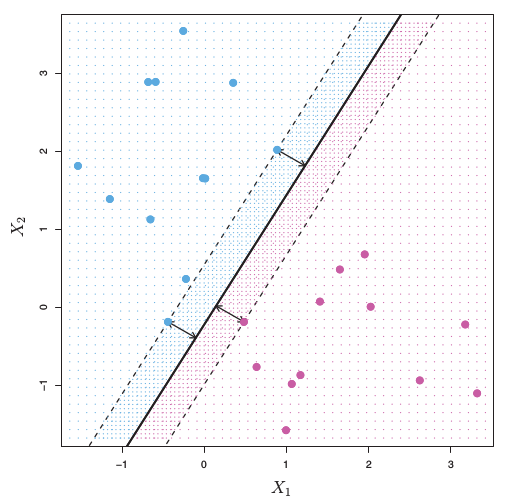
\includegraphics[width=1\textwidth]{conclusion/graphics/svm}

\emph{\footnotesize{}Explorar m�todos SVM (Support Vector Machine)
o ANN (Artificial Neural Networks)}{\footnotesize \par}
\onslide<3> 

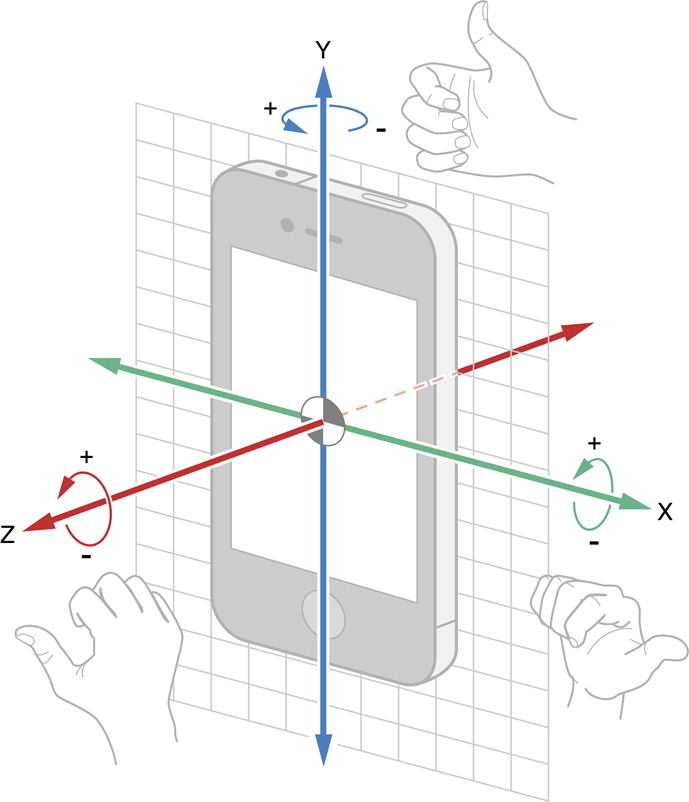
\includegraphics[width=1\textwidth]{conclusion/graphics/gyro}

\emph{\footnotesize{}Orientaci�n del dispositivo}{\footnotesize \par}
\onslide<4> 
\begin{center}

\includegraphics[width=1\textwidth]{conclusion/graphics/activities}
\par\end{center}

\begin{center}
\emph{\footnotesize{}Acciones diarias}
\par\end{center}{\footnotesize \par}
\onslide<5> 
\begin{center}
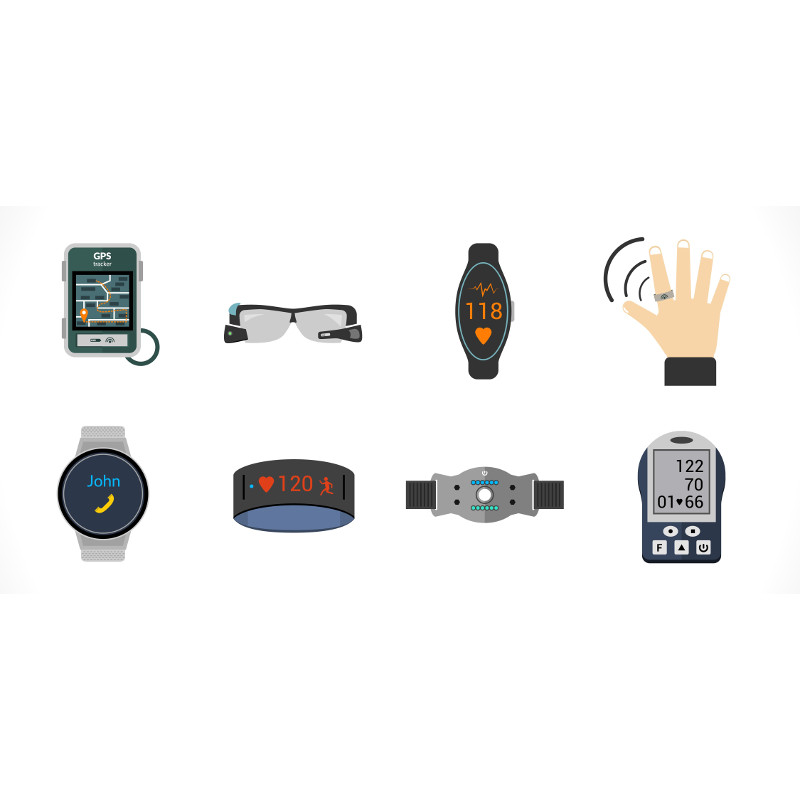
\includegraphics[width=1\textwidth]{conclusion/graphics/wear}
\par\end{center}

\emph{\footnotesize{}Accesorios como Smartwatch, Smartband, entre
otros}{\footnotesize \par}
\end{overprint}
\end{columns}

\end{frame}
%
\begin{frame}[t]{Conclusi�n}

\framesubtitle{Congresos y presentaciones}

\setlength\itemsep{1em}
\begin{itemize}
\item ICDE 2018 - 34th IEEE International Conference on Data Engineering
- Paris, Francia - \emph{(Pendiente)}
\item MobiSys 2018 - The 16th ACM International Conference on Mobile Systems,
Applications, and Services - Munich, Alemania - \emph{(Pendiente)}.
\end{itemize}
\end{frame}
%
\begin{frame}
\begin{center}

\includegraphics[width=0.8\textwidth]{conclusion/graphics/thanks}
\par\end{center}

\begin{center}
\structure{\begin{center}
Por su atenci�n!
\par\end{center}}
\par\end{center}
\end{frame}




\end{document}
